\chapter{Постановка требований и функциональности проекта}\label{ch:ch2}
\section{Описание бизнес-ролей}\label{sec:ch2/sec1}

\begin{table} [htbp]%
    \centering
    \begin{threeparttable}% выравнивание подписи по границам таблицы
      \caption{Список бизнес-ролей}
      \label{tab:test2}% label всегда желательно идти после caption
      \renewcommand{\arraystretch}{1.5}%% Увеличение расстояния между рядами, для улучшения восприятия.
      \begin{SingleSpace}
        \begin{tabular}{@{}@{\extracolsep{20pt}}llll@{}} %Вертикальные полосы не используются принципиально, как и лишние горизонтальные (допускается по ГОСТ 2.105 пункт 4.4.5) % @{} позволяет прижиматься к краям
            \toprule     %%% верхняя линейка
              Бизнес-роль & \centering Функции & \\
            \midrule %%% тонкий разделитель. Отделяет названия столбцов. Обязателен по ГОСТ 2.105 пункт 4.4.5
              Клиент &\centering Оформление заказа и эксплуатация виртуальных машин & \\
              Оператор  &\centering ОБработка запросов и инцидентов от клиентов. Заказ и проверка отчётов. & \\
              Администратор &\centering  Настройка и поддержка работоспособности системы и системы виртуализации. Работа с инцидентами.& \\
            \bottomrule %%% нижняя линейка
        \end{tabular}%
      \end{SingleSpace}
    \end{threeparttable}
\end{table}

\section{Функциональные требования}\label{sec:ch2/sec2}
\subsection{Основные требования}\label{sec:usecase_umls}
Система должна соотвествовать следующим требованиям:
\begin{itemize}
  \item производить накопление и хранение в базе данных всей полученной информации
  \item простой пользовательский интерфейс
  \item позволять оформлять заказы пользователям
  \item позволять пользователям производить простые операции (выключение, перезагрузка и включение) с вм через веб-интерфейс
  \item создавать в системе виртуализации ВМ с указанной пользователем конфигурацией
  \item позволять формировать отчёты по заказам
\end{itemize}

\subsection{Диаграммы прецедентов}\label{sec:usecase_umls}
На рисунке~\ref{fig:umls_register_ucesace} показан сценарий регистрации нового клиента.
\begin{figure}[ht]
  \centerfloat{
    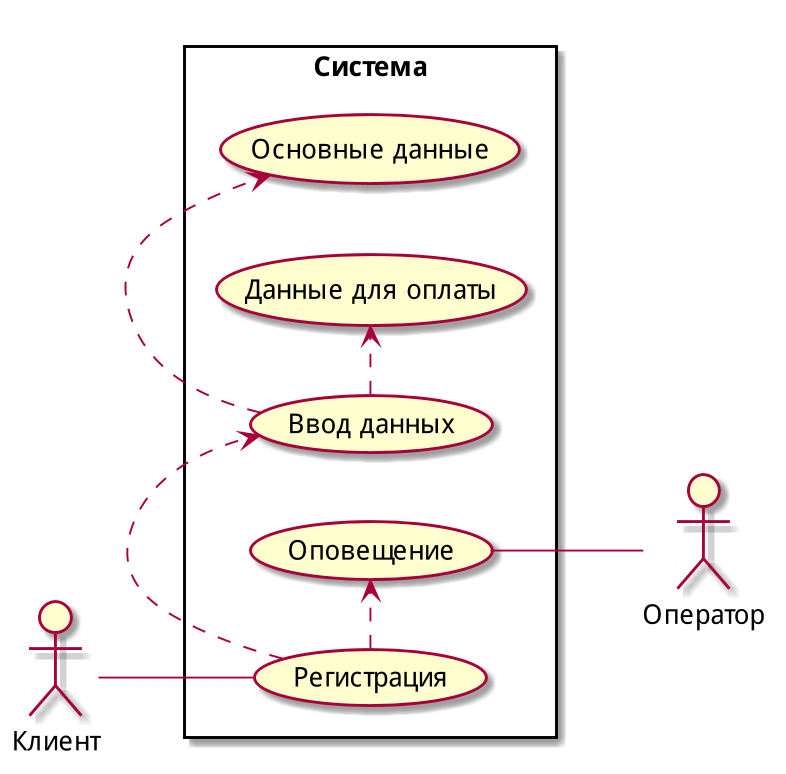
\includegraphics[scale=0.27]{umls/register_ucesace}
  }
  \caption{Сценарий регистрации клиента.}\label{fig:umls_register_ucesace}
\end{figure}

На рисунке~\ref{fig:umls_make_order_usecase} показан сценарий оформления заказа клиентом.
\begin{figure}[ht]
  \centerfloat{
    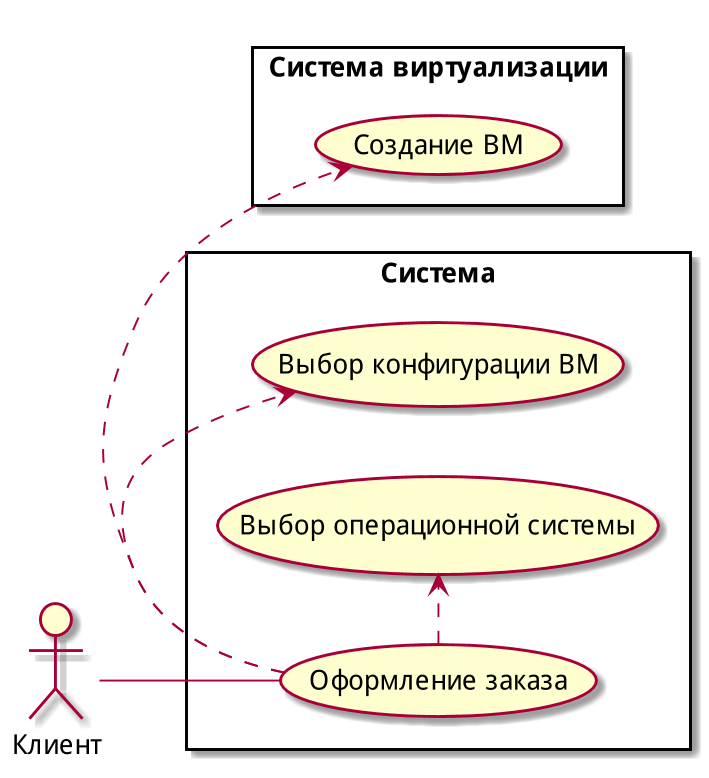
\includegraphics[scale=0.27]{umls/make_order_usecase}
  }
  \caption{Сценарий создания заказа.}\label{fig:umls_make_order_usecase}
\end{figure}

На рисунке~\ref{fig:umls_report_request_usecase} показан сценарий оформления заказа клиентом.
\begin{figure}[ht]
  \centerfloat{
    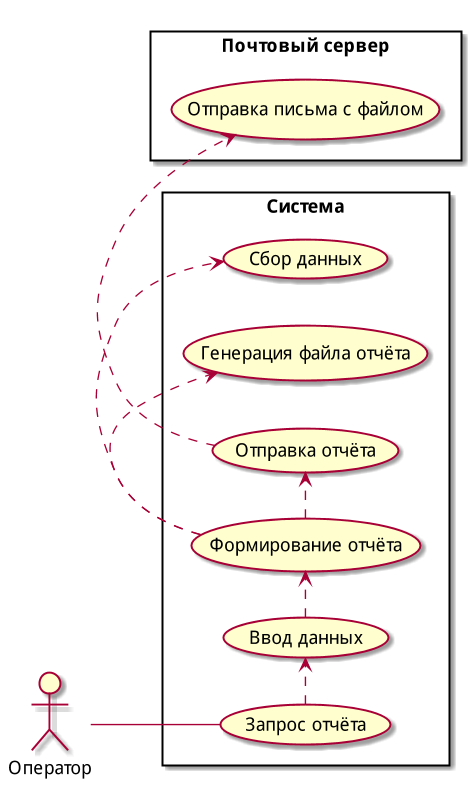
\includegraphics[scale=0.27]{umls/report_request_usecase}
  }
  \caption{Сценарий создания заказа.}\label{fig:umls_report_request_usecase}
\end{figure}

\section{Нефункциональные требования}\label{sec:ch2/sec3}
Система должна обладать следующими качествами:
\begin{itemize}
  \item используется язык Ruby
  \item используется фреймворк Ruby on Rails
  \item используется СУБД PostgreSQL
  \item используется Sidekiq для фоновых задач
  \item система разрабатывается для ОС семейства *nix
  \item используется сервер unicorn
  \item используется nginx в роли реверс-прокси
  \item используется система виртуализации OpenStack
  \item оплата производится через систему Яндекс.Касса
\end{itemize}
